\section*{Editorial} 
\label{editorial}
\NewsAuthor{Horst JENS}

%\begin{wrapfigure}{r}{2.0cm}
\begin{center}
\includegraphics[width=0.8\linewidth]{editorial/horst2011mitdoppeltux.jpg}\\ 
\footnotesize{Horst JENS [1]}
\end{center}   
%\end{wrapfigure}
\textbf{Wenn Sie dieses editorial zu Ende lesen verrate ich [1] Ihnen wo sich die Werbung im \textit{R.I.S.-Journal} versteckt, warum Sie zu viel daf\"ur gezahlt haben, wof\"ur der Name \textit{R.I.S.} steht und was es mit den \textit{Creativ-Commons Lizenzen} auf sich hat. Und wie Sie mich dazu bringen an in Ihrer Schule einen Game-Programming Workshop zu veranstalten.} 

%\begin{center}
%\includegraphics[width=3cm]{horst2011mitdoppeltux.jpg}\\
%\footnotesize{Horst JENS, Herausgeber, Chefredakteur etc. Bildrechte: cc-by-sa [1]}
%\end{center}

\subsection*{Wie alles begann...}
Genau vor einem Jahr, zum Jahreswechsel 2012 auf 2013, hatte ich die Idee um mein Geschäft (Programmierkurse für Jugendliche)\footnote{Open Source Game Programming - Kurse für Kinder, Jugendliche und Schulen: Firma \href{http://spielend-programmieren.at}{\textit{spielend-programmieren}} [1]} anzukurbeln anstatt der üblichen Plakate, Flugzettel und Inserate gleich eine eigene Zeitschrift herauszubringen um sie an Schulen als Werbemittel zu verteilen. Genialerweise ist es teurer ein einziges Inserat in einer uninteressanten Zeitung zu bezahlen als eine interessante Zeitung ohne uninteressante Inserate zu erstellen. Weiter unten verrate ich wie Sie das R.I.S. Journal für Ihre eigenen Zwecke nutzen können.

Diverse Projekte verzögerten mein Vorhaben bis es endlich zum Jahreswechsel 2013 / 2014 so weit war: Ich hatte genug Zeit um die bisher gesammelten Artikel noch einmal durchzuarbeiten, die Layoutsprache {\large \LaTeX} zu lernen und sehr viele E-Mails zu schreiben um weltweit nach Übersetzungs- und Abdruck-Genehmigungen zu fragen. 

\subsection*{Lausch- und Lesefutter}
Die meisten der Artikel dieser Ausgabe des RIS-Journals habe ich vom Englischen ins Deutsche übersetzt. Viel weniger Artikel als ursprünglich geplant sind von mir selbst... freuen Sie sich auf die nächste Ausgabe des RIS-Journals dort werden mehr Artikel von mir drin sein. Werfen Sie bis dahin einen Blick auf die \href{http://spielend-programmieren.at/de:tutorials:start}{\textit{Tutorials meiner Homepage [2]}} oder in mein \href{http://thepythongamebook.com}{\textit{Python Game Book [3]}} bzw. hören Sie sich meinen \href{http://biertaucher.at}{\textit{wöchentlichen \textbf{Podcast} [4]}} an, dann wissen Sie recht gut welche Themen ich in den nächsten Ausgaben dieses Journals behandeln werde und über welche Themen ich an Ihrer Schule einen Workshop anbieten kann:

\subsection*{Meine Werbung...}
Warum ich an Ihrer Schule zeigen will was ich kann: Einerseits weil es (selten, aber doch) vorkommt dass Schulen mich direkt für einen Workshop bezahlen; vor allem aber weil ich dadurch Kunden für meine Programmierkurse [1] gewinnen kann. Bei \href{http://spielend-programmieren.at}{\textit{spielend-programmieren}} gibt es für Jugendliche jede Altersstufe Programmierkurse, sowohl während der Schulzeit als auch während der Ferien. Näheres erfahren Sie auf \href{http://spielend-programmieren.at}{\textit{meiner Homepage}} [1]!

\begin{center}

\includegraphics[width=0.5\linewidth]{editorial/editorial-tuxstick3.png}\\
\footnotesize{Logo der Firma spielend-programmieren: Tux mit Joystick}
\end{center}

\subsection*{...an Ihrer Schule}
Womit wir beim Sinn dieses Journals angelangt sind: Ich kann gerne in Ihrer Schule / für Ihre Organisation einen Workshop (bzw. eine Probestunde) zum Thema Open Source / Programmieren / Game Programming abhalten, kombinierbar mit beinahe jedem Unterrichtsfach \footnote{Sogar Turnstunden, und sogar ohne Computer. Am Liebsten sind mir Schulen mit gut bestücktem EDV-Saal} - kontaktieren Sie mich einfach per Email, Kontaktmöglichkeiten und Einzelheiten finden Sie auf meiner  meiner Homepage \href{http://spielend-programmieren.at}{\textit{spielend-programmieren.at}}.


\subsection*{Frei lizensiert}
Alle (übersetzten) Texte im RIS Journal sind frei lizensiert und auch fast alle Grafiken\footnote{bitte beachten Sie im Einzelfall die Bildunterschriften}. Da (zumindest die Texte) alle unter eine \textbf{Creative Commons cc-by-sa Lizenz} fallen können Sie diese Texte nicht nur im Unterricht beliebig (legal!) verteilen und verwenden sondern daraus auch ihre eigene Zeitschrift machen...mit Ihrer Werbung und mir Ihren eigenen, zusätzlichen Inhalten. Unter Beachtung folgender Bedingung:
\begin{itemize} 
\item Namensnennung (recognition): Sie müssen auf die Originalquelle verlinken / hinweisen. 
\item Weitergabe unter gleichen Bedingungen (share-alike): Die daraus entstehenden Artikeln oder Werke müssen ebenfalls cc-by-sa lizensiert sein und frei kopiert werden können.
\end{itemize}
Was Sie \emph{nicht} können ist eine \textbf{cc-by-sa} Lizenz rückgängig zu machen: meine Artikel bleiben frei lizensiert. Sie können trotzdem für Ihre Zeitschrift Geld verlangen, Sie können aber nicht verhindern dass die freien Artikeln kopiert werden. Sie dürfen keinen  Kopierschutz oder Copyright-Vermerk zu Inhalten des RIS Journals hinzufügen, davor schützt die \textbf{Creative-Commons Lizenz}. Womit wir beim Preis angelangt sind:

\subsection*{Preis}
Das RIS Journal wird immer kostenlos erhältlich sein (z.B. indem Sie die Online-Version herunterladen, ausdrucken und verteilen). Wobei es vollkommen in Ordnung ist das R.I.S.-Journal zu verkaufen: kostenlos ist ja nicht das selbe wie wertlos, und die \textbf{cc-by-sa Lizenz} erlaubt auch den Verkauf ausdrücklich. Sie können dieses R.I.S.-Journal nehmen und jemand anderem verkaufen, ich freue mich sogar darüber! Bitte schreiben Sie mir welchen Preis Sie erzielt haben. 

\subsection*{R.I.S. Journal ?}
Im Name Journal kommt steckt das Wort 'jour' (französich für Tag), gemeint ist eine tägliche bzw. tagesaktuelle Zeitschrift. Sie halten Ausgabe 001 in der Hand und ich habe über ein Jahr dafür gebraucht... realistischerweise habe ich vor etwa vier Ausgaben pro Jahr herausbringen, später vielleicht mehr. R.I.S. steht für \textbf{R}emix - \textbf{I}mprove - \textbf{S}hare und fasst recht gut das Gedankengebäude der freien Software / Open Source Welt zusammen, nämlich die vier Grundfreiheiten der \textbf{gpl-Lizenz}: Die Freiheiten ein Werk (z.B. Software) 
\begin{itemize}
\item zu nutzen (use, Remix)
\item zu verbessern (modify, Improve)
\item zu verbreiten (Share)
\item zu studieren (study) (davon zu lernen, Zugriff auf die Quelldateien /Baupläne zu haben)
\end{itemize}

Diese vier Grundfreiheiten bilden das Fundament der Welt der freien Software (Free/libre Open Source Software) und führen zu einer Kultur (\href{http://en.wikipedia.org/wiki/Hacker_ethic}{\textbf{Hackerethik}}) des miteinander Teilens (von Wissen), des weltweiten Zusammenarbeitens\footnote{die Open Source Welt kann mehr Programmierer auf eine Aufgabe konzentrieren als jede einzelne Firma}. Diese Kultur ist der Grund warum heute technisches Spitzenprodukte frei erhältlich sind wie etwa das Betriebssystem \textbf{Gnu/Linux}, die Grafiksoftware \textbf{Gimp} oder die 3D-Software \textbf{Blender}. Diese Kultur ist der Grund warum tausende Freiwillige die größte jemals verfügbare, creativ-commons lizensierte Enzyklopädie erschaffen haben (\textbf{Wikipedia}) an der jeder mitarbeiten kann. Diese Kultur ist der Grund warum sich weltweit Leute zusammentun um ein freies Hochglanzmagazine wie \href{http://gimpmagazine.org/}{\textit{Gimpmagazine.org}} zu erschaffen oder gemeinsam an einem freien Film wie \href{http://www.sintel.org/}{\textit{Sintel [5]}} zu arbeiten. \\

\begin{center}

\includegraphics[width=\linewidth]{editorial/editorial-sintel.png}\\
\footnotesize{Szene aus dem Blender-Film \emph{Sintel}. Bildrechte: [5]}
\end{center}

Diese Kultur bleibt nicht auf immaterielle Güter wie Software beschränkt sondern betrifft z.B. dank austauschbarer Pläne für 3D Drucker mehr und mehr Bereiche außerhalb der klassischen Software-Industrie. Werfen Sie einmal einen Blick auf den Blog von \href{http://opensourceecology.org/}{\textbf{Open Source Ecology}}: erdverbundener geht es nicht mehr. 

\subsection*{Mitmachen}
Diese freien Inhalte und die damit verbundene Kultur bekannt zu machen und zu fördern, speziell in Schulen, ist mein Ziel für das R.I.S. Journal. Ich wünsche viel Spaß beim Lesen. Bitte schreiben Sie mir was Ihnen gefallen hat, und vor allem: Wenn Ihnen ein Artikel nicht gefallen hat, schreiben Sie mir einen besseren Artikel für die nächste Ausgabe! Wie Sie sehen können brauche ich auch dringend Grafiker, Übersetzter, Redakteure, Korrekturleser und Leute die sich mit {\large \LaTeX} auskennen. 

\subsection*{Spenden}
Auch wenn Sie das RIS Journal kostenlos downloaden, ausdrucken und verbreiten dürfen bedeutet dies keinesfalls dass ich mich gegen Spenden wehre. Wenn Sie mir absolut keinen Auftrag für einen Programmierkurs geben wollen sondern mir lieber einfach so Geld zukommen lassen wollen, ganz ohne Gegenleistung:


Banküberweisung: Bitte schreiben Sie in den Buchungstext 'Spende für RIS-Journal 001':
\texttt{Kontoinhaber: Horst JENS \\
IBAN: AT69 6000 0000 7515 9553\\
BIC: OPSKATWW} \\
Selbstverständlich freue ich mich auch über \textbf{Bitcoins}:\\
\texttt{1CZ4 dCgF 8sMX Zmbd wjiR 9nPM 52b4 QSxa nb}
Sowie über \textbf{Flattr} - Spenden: \url{http://goo.gl/5nJz6y}
\begin{center}

\includegraphics[width=0.49\linewidth]{editorial/editorial-bitcoin-qr.jpg} 

\includegraphics[width=0.49\linewidth]{editorial/editorial-flattr-qr.png}
\footnotesize{Bitcoin-Adresse (links) und Flattr Adresse (rechts) von Horst JENS}
\end{center}
%Sowie über \textbf{Flattr} - Spenden: \url{http://goo.gl/5nJz6y}
%\begin{center}
%
\includegraphics[width=2.5cm]{editorial-flattr-qr.png}\\
%\footnotesize{Flattr Url für Mikrospenden}
%\end{center}

%\subsection*{Quelldateien}

%Alle Dateien die für diese Zeitschrift verwendet wurden (und viele Dateien die nicht verwendet wurden) finden Sie verlinkt unter folgender URL: \href{http://spielend-programmieren.at/de:ris:001:start}{spielend-programmieren.at/de:ris:001:start}.

\subsection*{Gliederung}
Bis ich eine bessere Layout Idee habe ist jeder Artikel folgendermaßen aufgebaut:
\begin{itemize}
\item Anrisstext, \textbf{fett gedruckt} wo kurz erklärt wird worum es in dem Artikel geht damit Sie entscheiden können ob Sie ihn lesen wollen oder nicht.
\item Der Artikeltext selbst, inklusive Bildern, \textbf{fett geschriebenen Fachbegriffen} und \textit{kursiven} \href{http://spielend-programmieren.at}{\textit{Links zu Web-Adressen (URL)}} [1], mit Zahlen in eckigen Klammern dahinter (siehe Quellen) falls die URL nicht selbst-erklärend ist. In der Online-Version ist die URL direkt anklickbar.
\item Fachbegriffe (sofern vorhanden) einzeln erklärt. Falls die Website zum Fachbegriff nicht dem gleichlautendem Wikipedia-Artikel entspricht wird sie \texttt{extra angegeben}.
\item Download \& Feedback: Link zum Direkt-Download des Artikels, falls vorhanden Link zur Audio-Datei (\textbf{Podcast}). Falls vorhanden E-Mail Adresse der Autoren.
\item Lizenzangabe diese Lizenzangabe bezieht sich immer auf den (in Deutsche übersetzten) Text. Bilder und Originaltexte können abweichende Lizensierungen haben ! 
\item Quellen: Alle Links und Quellenangaben dieses Artikels
\end{itemize}

\subsection*{Fachbegriffe:}

~~~\textbf{cc-by-sa} creative-commons, recognition, share-alike Lizenz:  Namensnennung, Weitergabe unter gleichen Bedingungen. Siehe auch weiter unten \\

\textbf{gpl} General Public License, ermöglicht die 4 Grundfreiheiten \emph{use, study, share, improve} im Bereich Software. Sie wurde von Richard Stallman erfunden und wird weltweit von der Free Software Foundation (Europa: \href{http://fsfe.org/}{\textit{fsfe.org}}) gefördert und durchgesetzt. Für Dokumentationen, Text, Musik und künstlerische Werke hat sich die Creative Commons Lizenz cc-by-sa bewährt. \\

%\begin{wrapfigure}{l}{2.0cm}
\textbf{Hackerethik} Laut Steven Levy's Buch \href{http://www.amazon.de/gp/product/1449388396/ref=as_li_ss_tl?ie=UTF8&camp=1638&creative=19454&creativeASIN=1449388396&linkCode=as2&tag=spielendprogr-21}{\textit{Hackers. 25th Anniversary Edition: Heroes of the Computer Revolution}}\\ 
\begin{center}
\href{http://www.amazon.de/gp/product/1449388396/ref=as_li_ss_tl?ie=UTF8&camp=1638&creative=19454&creativeASIN=1449388396&linkCode=as2&tag=spielendprogr-21}{

\includegraphics[width=0.4\linewidth]{editorial/editorial-hackersqrcode.png} 
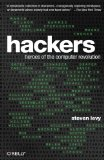
\includegraphics[width=0.4\linewidth]{editorial/editorial-hackers.jpg}}\\
\footnotesize{Bildrechte: Amazon Partner Programm [8]}
\end{center}
geht es bei der Hackerethik um folgende Werte:
%\end{wrapfigure}
\begin{itemize}
\item Free access: Zugang zu Computern soll frei sein
\item Sharing: Information soll frei sein
\item Decentralization: Misstraue Autorität (Behörden) - fördere Dezentralisierung
\item Openness: Beurteile Hacker nach deren Taten, nicht nach deren Zeugnissen
\item World Improvement: Du kanns Kunst und Schönheit mit dem Computer erschaffen
\item World Improvement: Computer können Dein Leben verbesseren
\end{itemize}

\textbf{Gnu/Linux} auch einfach nur Linux genannt, zum großen Leidwesen von Richard Stallman. Ein freies Betriebssystem für Computer. Steckt u.a. in Ihrem Android-Smartphone. Das Maskottchen von Linux, den Pinguin Tux, haben Sie sicher schon gesehen. \\

\textbf{Podcast} Eine Radiosendug (cast) welche als mp3 Datei via Internet gesendet wird und per Computer oder mp3-Player (iPod) angehört wird. \\

\textbf{Wikipedia} Lesen Sie einmal die Lizenzinformation eines beliebigen Wikipedia-Artikels ! \\

\href{http://opensourceecology.org/}{\textbf{Open Source Ecology}} [6]: Eine Gruppe von open-source begeisterten  Landfreaks die an einem "Global Village Construction Set" werkeln: vom Ziegelschneider über den Traktor bis zum Fertighaus werden alle Pläne und Erfahrungen über das Internet verteilt, frei lizensiert und weltweit nachgebaut und verbessert.\\

\textbf{Flattr} eine Micro-payment Dienst der es erlaubt sehr kleine Beträge  zu spenden (z.B. einen Zwanzigstel von einem Cent). Auf \url{http://flattr.com} erfahren Sie mehr darüber.\\

\textbf{Bitcoins} Bitcoins sind elektronisches Geld welches sich ohne Überweisungsgebühr überweisen lässt, in beliebig kleinen Beträgen. Ich verspreche Ihnen einen ausführlichen Artikel zum Thema Bitcoins in einer der nächsten Ausgaben des R.I.S.-Journals. Bis dahin hören Sie doch einmal in den \textbf{Podcast}  \href{http://www.bitcoinupdate.com/}{\textit{Bitcoin-Update [7]}} hinein!

\subsection*{Download, Feedback:}
\footnotesize{
Download: Ordner \texttt{editorial} \Mundus\ \href{http://spielend-programmieren.at/risjournal/001}{spielend-programmieren.at/risjournal/001}\\
Startseite:\\
\href{http://spielend-programmieren.at/de:ris:001}{spielend-programmieren.at/de:ris:001}\\ 
\Letter\: horst.jens@spielend-programmieren.at}
\normalsize
%\url{http://goo.gl/1FozRo} \\

\subsection*{Lizenz, Quellen} 
\begin{wrapfigure}{l}{2.0cm}

\includegraphics[width=2cm]{editorial/ccbysa88x31.png}
\end{wrapfigure}
Dieses Material steht unter der Creative-Commons-Lizenz Namensnennung - Weitergabe unter gleichen Bedingungen 4.0 International. Um eine Kopie dieser Lizenz zu sehen, besuchen Sie \url{http://creativecommons.org/licenses/by-sa/4.0/deed.de}.

\textbf{Quellen:} \\
{[}1{]} \href{http://spielend-programmieren.at}{Spielend-Programmieren.at} \\
{[}2{]} \href{http://spielend-programmieren.at/de:tutorials:start}{http://goo.gl/0X37fd} \\
{[}3{]} \href{http://thepythongamebook.com}{ThePythonGameBook.com} \\
{[}4{]} \href{http://biertaucher.at}{Biertaucher.at} \\
{[}5{]} \href{http://www.sintel.org/}{Sintel.org} \\
{[}6{]} \href{http://opensourceecology.org/}{OpenSourcEecology.org} \\
{[}7{]} \href{http://www.bitcoinupdate.com/}{BitcoinUpdate.com} \\
{[}8{]} \href{http://www.amazon.de/gp/product/1449388396/ref=as_li_ss_tl?ie=UTF8&camp=1638&creative=19454&creativeASIN=1449388396&linkCode=as2&tag=spielendprogr-21}{goo.gl/EAkg5Q} \\










